\documentclass{article}
\usepackage{a4}
\usepackage{bm}
\usepackage{fullpage}
\usepackage{amsmath}
\usepackage{graphicx}
\usepackage{url}
\parindent 0pt
\parskip 6pt

\newcommand{\outdeg}{\mbox{\sf outdeg}}
\newcommand{\indeg}{\mbox{\sf indeg}}
\newcommand{\card}[1]{\mid\!#1\!\mid}
\newcommand{\tc}{\mbox{\sf tc}}
\newcommand{\tr}{\mbox{\sf tr}}
\newcommand{\ku}{\mbox{\sf ku}}

\newcommand{\cb}{\bm{c}}
\newcommand{\kb}{\bm{k}}
\newcommand{\A}{\bm{A}}
\newcommand{\E}{\bm{E}}
\newcommand{\I}{\bm{I}}
\newcommand{\one}{\bm{1}}
\newcommand{\vb}{\bm{v}}
\newcommand{\W}{\bm{W}}
\newcommand{\tp}[1]{#1\!^{\top}}
\newcommand{\AT}{\tp{\A}}

\begin{document}
{\bf Transitive Credit}  (subsumes previous document)

We take the citation graph to be a graph $(V,E)$ with $E\subset
V\times V$.  The edge $(v_i,v_j)$ represents the fact that $v_i$ cites
$v_j$.  We shall assume that $(V,E)$ is devoid of cycles; it is a
d.a.g.

The in- and out-degree of a node $n$ are respectively defined as
$\indeg(n) = \card{\{m \mid (m,n) \in V\}}$ and\\
$\outdeg(n) = \card{\{m \mid (n,m) \in V\}}$.  The normal citation
count or {\em credit} for a node $n$ is simply $\indeg(n)$. 

We now consider a model in which credit can be transferred from one
node to another -- along the edges. Each node gives up some of its
incoming credit to its (out-) neighbors.   We define the following
quantities:

\begin{tabular}{rcl}
  $\tc(n)$ & -- &  the total credit accumulated by a node,\\
  $\ku(n)$ & -- & the credit kept by a node -- its kudos, and\\
  $\tr(n,m)$ & -- &  the credit transferred along the edge $(n,m)$.
\end{tabular}

Each node receives the normal citation credit of $1$ for each incoming edge.
It also receives credit transfer from the nodes that cite it along
each such edge:
$$\tc(n) = \Sigma_{(m,n)\in E} 1+\tr(m,n)$$

The kudos is the amount of credit a node keeps, which is the totel
credit less than the amount of credit that flows along the out-edges f
that node:
$$\ku(n) = \tc(n)  - \Sigma_{(n,m)\in E} \tr(n,m)$$

{\bf Prop}. $\Sigma_{n\in N} \ku(n) = \card{E}$

This is something that I think we need: that redistributing credit
does not create or diminish credit.

The question is now how to define $\tr$.  The simplest method is, I
think, for every node to give up a fraction $\alpha$ of its credit
keep the remaining $(1-\alpha)$ for itself a fraction $\alpha$. It also
distributes the outgoing fraction {\em equally} over the outgoing edges
\[
\begin{array}{rcl}
  \tr(n,m) &  = & \frac{\alpha}{\outdeg(n)}\tc(n)\\
  \ku(n) & = & (1-\alpha)\tc(n)
\end{array}
\]



This has the property that it satisfies the conditions for $tc$
above.   In the case that $\alpha = 0$ it is the normal citation
count. When $\alpha=1$ the credit piles up at the terminal nodes of
the d.a.g.

Of course, $\alpha$ does not have to be the same for each node, nor
does the distribution of credit over the cited nodes need to be
uniform, but maybe this is a starting point.

\newpage

{\bf A more general formulation}

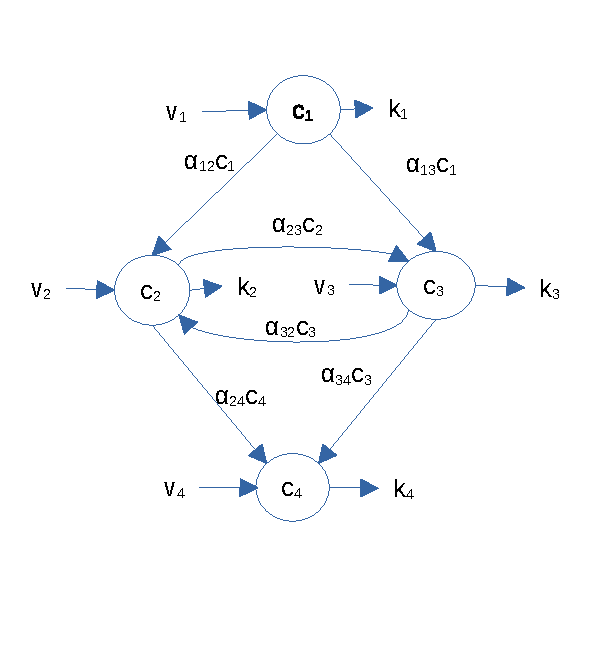
\includegraphics[scale=0.8]{pic1.pdf}

In this formulation we allow each node to decide how much credit it keeps and how
much it gives away.   We also allow cycles.
Consider node $2$ in the picture above.  It receives credit from nodes
$1$ and $3$; and rather assuming that it receives one unit of credit
for each citation edge, we shall simply assume that it receives an
amount $v_2$.  It {\em gives} credit to nodes $3$ and $4$.  It takes the
total received  $c_2$, sends  $\alpha_{23}c_2$ to node
$2$, $\alpha_{24}c_2$ to node $4$ and keeps the remainder,
$(1 -(\alpha_{23}+\alpha_{24}))c_2$ to itself as its kudos, $k_2$. So we
have
$$c_2 = \alpha_{12}c_1 + \alpha_{32}c_3 + v_2  \ \ \mbox{and}
\ \ k_2 = c_2 -(\alpha_{23} + \alpha_{24})c_2$$

We can write down all such equations as matrix operations:


\[
\left[
\begin{array}{c}
    c_1 \\ c_2 \\ c_3 \\ c_4
\end{array}
\right]
=
\left[
\begin{array}{cccc}
  0          & 0          & 0           & 0 \\
  \alpha_{12} & 0          & \alpha_{32} & 0 \\
  \alpha_{13} & \alpha_{23} & 0          & 0 \\
  0          & \alpha_{24} & \alpha_{34} &  0
\end{array}
\right]
\left[
\begin{array}{c}
  c_1 \\  c_2\\  c_3\\  c_4
\end{array}
\right]
+
\left[
\begin{array}{c}
  v_1 \\  v_2\\  v_3\\  v_4
\end{array}
\right]
\]

and
\[
\left[
  \begin{array}{c}
    k_1 \\ k_2 \\ k_3 \\ k_4
  \end{array}
  \right]
=
\left[
  \begin{array}{c}
    c_1 \\ c_2 \\ c_3 \\ c_4
  \end{array}
  \right]
-
\left(\left[
  \begin{array}{cccc}
    0     & \alpha_{12} & \alpha_{13}  & 0          \\
    0     & 0          & \alpha_{23}  & \alpha_{24} \\
    0     & \alpha_{32} & 0           & \alpha_{34} \\
    0     & 0          & 0           & 0           
  \end{array}
  \right]
\left[
  \begin{array}{c}
    1 \\ 1 \\ 1 \\ 1
  \end{array}
  \right]
\right)
\times
\left[
  \begin{array}{c}
    c_1 \\ c_2 \\ c_3 \\ c_4
  \end{array}
  \right]
\]




where $+$ and $\times$ are pointwise operations on vectors or matrices
of the same dimension. Writing $\cb$, $\kb$, $\vb$ and $\one$ for the credit, kudos, input
``citation'' and unit vectors; and writing $\A$ for the transfer weights matrix  we have:
% 
\begin{equation}\label{ineq}
  \cb = \AT\cb+\vb
\end{equation}
% 
\begin{equation}\label{outeq}
  \kb = \cb - (\A\one)\times\cb
\end{equation}

The {\em total} credit being input is $\Sigma_{i=1}^nv_i$ or
$\tp{\one}\vb$, which, using \ref{ineq} and \ref{outeq} and noting
that the inner or ``dot'' product $\bm{x}\cdot\bm{y}$ is
$\tp{\one}(\bm{x}\times\bm{y})$, gives\footnote{\url{https://en.wikipedia.org/wiki/Transpose}}

\[
\tp{\one}\vb = \tp{\one}\cb - \tp{\one}\AT\cb =
\tp{\one}\cb -\tp{(\A\one)}\cb = \tp{\one}\cb - (\A\one)\cdot \cb =
\tp{\one}\cb - \tp{\one}(\A\one)\times\cb = \tp{\one}\kb
\]

Which is just a sanity check on what goes in must come out and {\em
  vice versa} -- even
when there are multiple solutions for the credit vector $\cb$. When do
we have multiple solutions?  If there are multiple solutions, is there
one that is minimal in some sense?!ev


Now, expanding, we have $\cb = (\I + \AT + (\AT)^2 + (\AT)^3 + \ldots)\vb$ and,
assuming the series  $\I + \AT + (\AT)^2 + (\AT)^3 + \ldots$ converges to
$\W$, we have $\I +\AT\W = \W$. 



\end{document}
 
